%%
%% This is file `sample-sigplan.tex',
%% generated with the docstrip utility.
%%
%% The original source files were:
%%
%% samples.dtx  (with options: `sigplan')
%% 
%% IMPORTANT NOTICE:
%% 
%% For the copyright see the source file.
%% 
%% Any modified versions of this file must be renamed
%% with new filenames distinct from sample-sigplan.tex.
%% 
%% For distribution of the original source see the terms
%% for copying and modification in the file samples.dtx.
%% 
%% This generated file may be distributed as long as the
%% original source files, as listed above, are part of the
%% same distribution. (The sources need not necessarily be
%% in the same archive or directory.)
%%
%% Commands for TeXCount
%TC:macro \cite [option:text,text]
%TC:macro \citep [option:text,text]
%TC:macro \citet [option:text,text]
%TC:envir table 0 1
%TC:envir table* 0 1
%TC:envir tabular [ignore] word
%TC:envir displaymath 0 word
%TC:envir math 0 word
%TC:envir comment 0 0
%%
%%
%% The first command in your LaTeX source must be the \documentclass command.
\documentclass[sigplan,screen]{acmart}
%% NOTE that a single column version is required for 
%% submission and peer review. This can be done by changing
%% the \doucmentclass[...]{acmart} in this template to 
%% \documentclass[manuscript,screen,review]{acmart}
%% 
%% To ensure 100% compatibility, please check the white list of
%% approved LaTeX packages to be used with the Master Article Template at
%% https://www.acm.org/publications/taps/whitelist-of-latex-packages 
%% before creating your document. The white list page provides 
%% information on how to submit additional LaTeX packages for 
%% review and adoption.
%% Fonts used in the template cannot be substituted; margin 
%% adjustments are not allowed.
%%
%% \BibTeX command to typeset BibTeX logo in the docs
\AtBeginDocument{%
  \providecommand\BibTeX{{%
    \normalfont B\kern-0.5em{\scshape i\kern-0.25em b}\kern-0.8em\TeX}}}

%% Rights management information.  This information is sent to you
%% when you complete the rights form.  These commands have SAMPLE
%% values in them; it is your responsibility as an author to replace
%% the commands and values with those provided to you when you
%% complete the rights form.
\setcopyright{acmcopyright}
\copyrightyear{2018}
\acmYear{2018}
\acmDOI{XXXXXXX.XXXXXXX}

%% These commands are for a PROCEEDINGS abstract or paper.
\acmConference[Conference acronym 'XX]{Make sure to enter the correct
  conference title from your rights confirmation emai}{June 03--05,
  2018}{Woodstock, NY}
%
%  Uncomment \acmBooktitle if th title of the proceedings is different
%  from ``Proceedings of ...''!
%
%\acmBooktitle{Woodstock '18: ACM Symposium on Neural Gaze Detection,
%  June 03--05, 2018, Woodstock, NY} 
\acmPrice{15.00}
\acmISBN{978-1-4503-XXXX-X/18/06}


%%
%% Submission ID.
%% Use this when submitting an article to a sponsored event. You'll
%% receive a unique submission ID from the organizers
%% of the event, and this ID should be used as the parameter to this command.
%%\acmSubmissionID{123-A56-BU3}

%%
%% The majority of ACM publications use numbered citations and
%% references.  The command \citestyle{authoryear} switches to the
%% "author year" style.
%%
%% If you are preparing content for an event
%% sponsored by ACM SIGGRAPH, you must use the "author year" style of
%% citations and references.
%% Uncommenting
%% the next command will enable that style.
%%\citestyle{acmauthoryear}

%%
%% end of the preamble, start of the body of the document source.
\begin{document}

%%
%% The "title" command has an optional parameter,
%% allowing the author to define a "short title" to be used in page headers.
\title{Trabalho Prático - IA}

%%
%% The "author" command and its associated commands are used to define
%% the authors and their affiliations.
%% Of note is the shared affiliation of the first two authors, and the
%% "authornote" and "authornotemark" commands
%% used to denote shared contribution to the research.
\author{Eric Azevedo de Oliveira}
\affiliation{%
 %% \institution{The Th{\o}rv{\"a}ld Group}
 %% \streetaddress{1 Th{\o}rv{\"a}ld Circle}
  \city{Belo Horizonte}
  \country{Brasil}}
\email{eric.azevedo@sga.pucminas.br}

\author{Felipe Nepomuceno Coelho}
\affiliation{%
 %% \institution{The Th{\o}rv{\"a}ld Group}
  %%\streetaddress{1 Th{\o}rv{\"a}ld Circle}
  \city{Belo Horizonte}
  \country{Brasil}}
\email{felipe.coelho.1265277@sga.pucminas.br}



\author{Iyan Lucas Duarte Marques}
\affiliation{%
 %%\institution{Rajiv Gandhi University}
%% \streetaddress{Rono-Hills}
 \city{Belo Horizonte}
 \country{Brasil}}
\email{ildmarques@sga.pucminas.br}


%%
%% By default, the full list of authors will be used in the page
%% headers. Often, this list is too long, and will overlap
%% other information printed in the page headers. This command allows
%% the author to define a more concise list
%% of authors' names for this purpose.
%%\renewcommand{\shortauthors}{Trovato and Tobin, et al.}

%%
%% The abstract is a short summary of the work to be presented in the
%% article.



%%
%% The code below is generated by the tool at http://dl.acm.org/ccs.cfm.
%% Please copy and paste the code instead of the example below.




%%
%% Keywords. The author(s) should pick words that accurately describe
%% the work being presented. Separate the keywords with commas.


%% A "teaser" image appears between the author and affiliation
%% information and the body of the document, and typically spans the
%% page.


%%
%% This command processes the author and affiliation and title
%% information and builds the first part of the formatted document.
\maketitle


\begin{figure}[h]
  \centering
  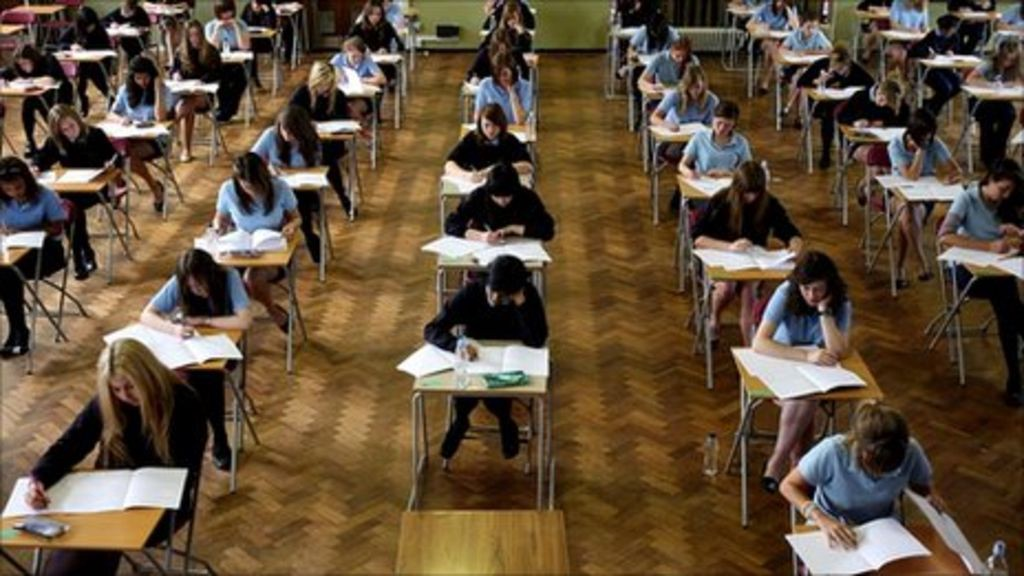
\includegraphics[width=\linewidth]{Estudante.png}
  \caption{Estudantes em sala de aula, realizando provas. (\url{https://medium.com/@JaskySingh/what-if-we-had-exams-everyday-well-everyone-would-be-better-off-f97919edeac}).}
  \Description{Estudantes em dia de prova.}
\end{figure}



\section{Introduction}
A base a ser utilizada será a "Students Performance in Exams" que pode ser encontrada em \url{https://www.kaggle.com/spscientist/students-performance-in-exams}. A base é composta por 8 atributos, sendo eles nominais, binários e numéricos:
\begin{itemize}
    \item Gender - Define o gênero da pessoa 
    \item Race/Ethnicity - Define a raça/etinia de uma pessoa em grupos separados entre A-D
    \item Parental level of education - Define o nível de educação dos pais da pessoa estudada
    \item Lunch - Define um padrão para a alimentação da pessoa estudada
    \item Test preparation course - Define se a pessoa estudada completou o curso de preparação
    \item Math score - Nota na matéria matemática
    \item Reading score - Nota em leitura
    \item Writing score - Nota em escrita
\end{itemize}

A base possui 1000 instâncias e não é um problema de classificação.

A base "Students Performance in Exams" retrata o impacto de certas características(Genêro, Raça, Nível de educação dos pais, Almoço e Realização do curso preparatório) que estão atreladas a cada aluno estudado em relação à sua performance em 3 matérias

%% Forma de  \cite{Ablamowicz07}





%%
%% The next two lines define the bibliography style to be used, and
%% the bibliography file.

\bibliographystyle{ACM-Reference-Format}
\bibliography{sample-base}

%%
%% If your work has an appendix, this is the place to put it.


\end{document}
\endinput
%%
%% End of file `sample-sigplan.tex'.
